\label{sec:signal_genstudy}
The relative composition of the diagrams shown in Figure~\ref{fig:ppTo4LG} in the signal sample was assessed in a generator level study.
The study is conducted on the four lepton channel, but the results can be generalised to the other two.
Two samples were generated at Leading Order EW ($\alpha_{\rm EW}^5 \, \alpS^0$) using \MADGRAPH.
The first is the inclusive production of four fermions and a photon, while the other constrains the intermediate vector boson state.

More precisely, the first sample simulates the process $\Pp\Pp \to 2\Pe 2\PGm \PGg$,
which in \MADGRAPH syntax corresponds to \verb|generate p p > e+ e- mu+ mu- a|.
The photon may be attached either to an initial- or final-state fermion line,
but not to a triple or quartic vertex since there are no suitable couplings in the SM for this final state.
The choice of a final state where the two lepton pairs have different flavour
excludes the interference from diagrams with the momenta of two leptons swapped.
The computed cross section is $0.075 \fbinv$.

The second sample forces the intermediate Z boson resonances $\Pp\Pp \to \PZ\PZ\PGg \to 2\Pe 2\PGm \PGg$,
using the syntax:
\begin{verbatim}
define ze = z
define zmu = z
generate p p > ze zmu a, ze > e+ e-, zmu > mu+ mu-
\end{verbatim}
In this case the photon is forced to be directly attached to an initial-state fermion line,
making this a sub-sample of the previous one.
The computed cross section is $0.026 \fbinv$. % $0.027 \fbinv$. % reason: the dRl>0.4 was not applied to this sample

Both samples were generated with the requirement that the leading (subleading) lepton has a transverse momentum larger than 20 (10)\GeV.
Every lepton is required to have $\pt^\Pl > 5\GeV$ and $|\eta^\Pl| < 2.5$,
while the photon must satisfy $\pt^\PGg > 20\GeV$ and $|\eta^\PGg| < 2.5$.
Additionally, the minimum separation between the photon and any of the four leptons must be $\DR(\Pl,\PGg) > 0.4$.

The distributions of the invariant mass of the same-flavour opposite-sign lepton pairs
and of the $\DR$ distance between the photon and the closest lepton
for the first and second sample are shown in Figure~\ref{fig:genstudy}.
From these plots it appears that in a sizeable fraction of FSR events the mass of one of the
$\Pl\Pl$ pairs is significantly lower than the \PZ peak.
It is also visible that most FSR photons are close to the parent lepton.
For these reasons, the triboson fiducial region, detailed in Section~\ref{sec:FSR_cut},
is defined using cuts on these variables.

\begin{figure}
  \centering\hfill
  \subfigure [Dilepton invariant mass] {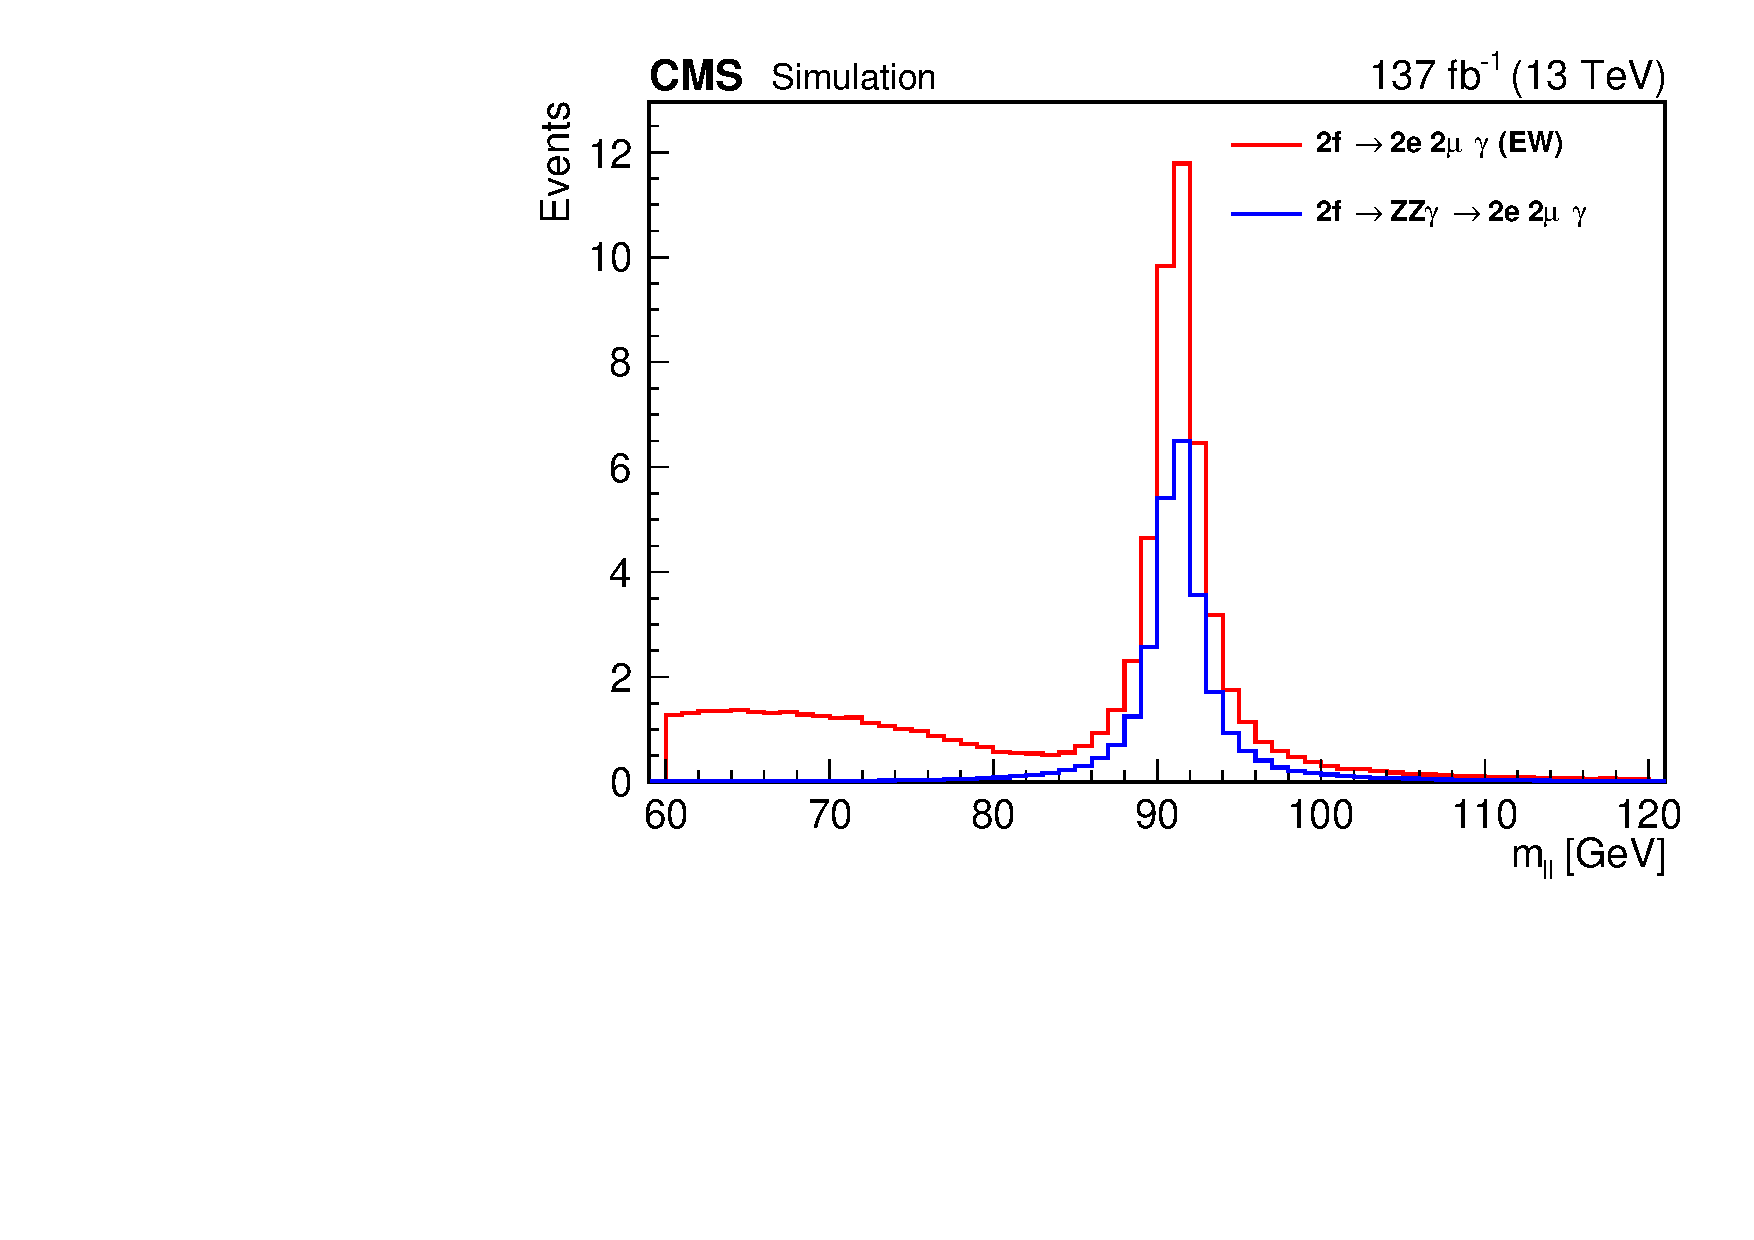
\includegraphics[width=.45\textwidth]{genstudy_mll.pdf}}\hfill
  \subfigure [Minimum $\DR$ between the \PGg and a lepton] {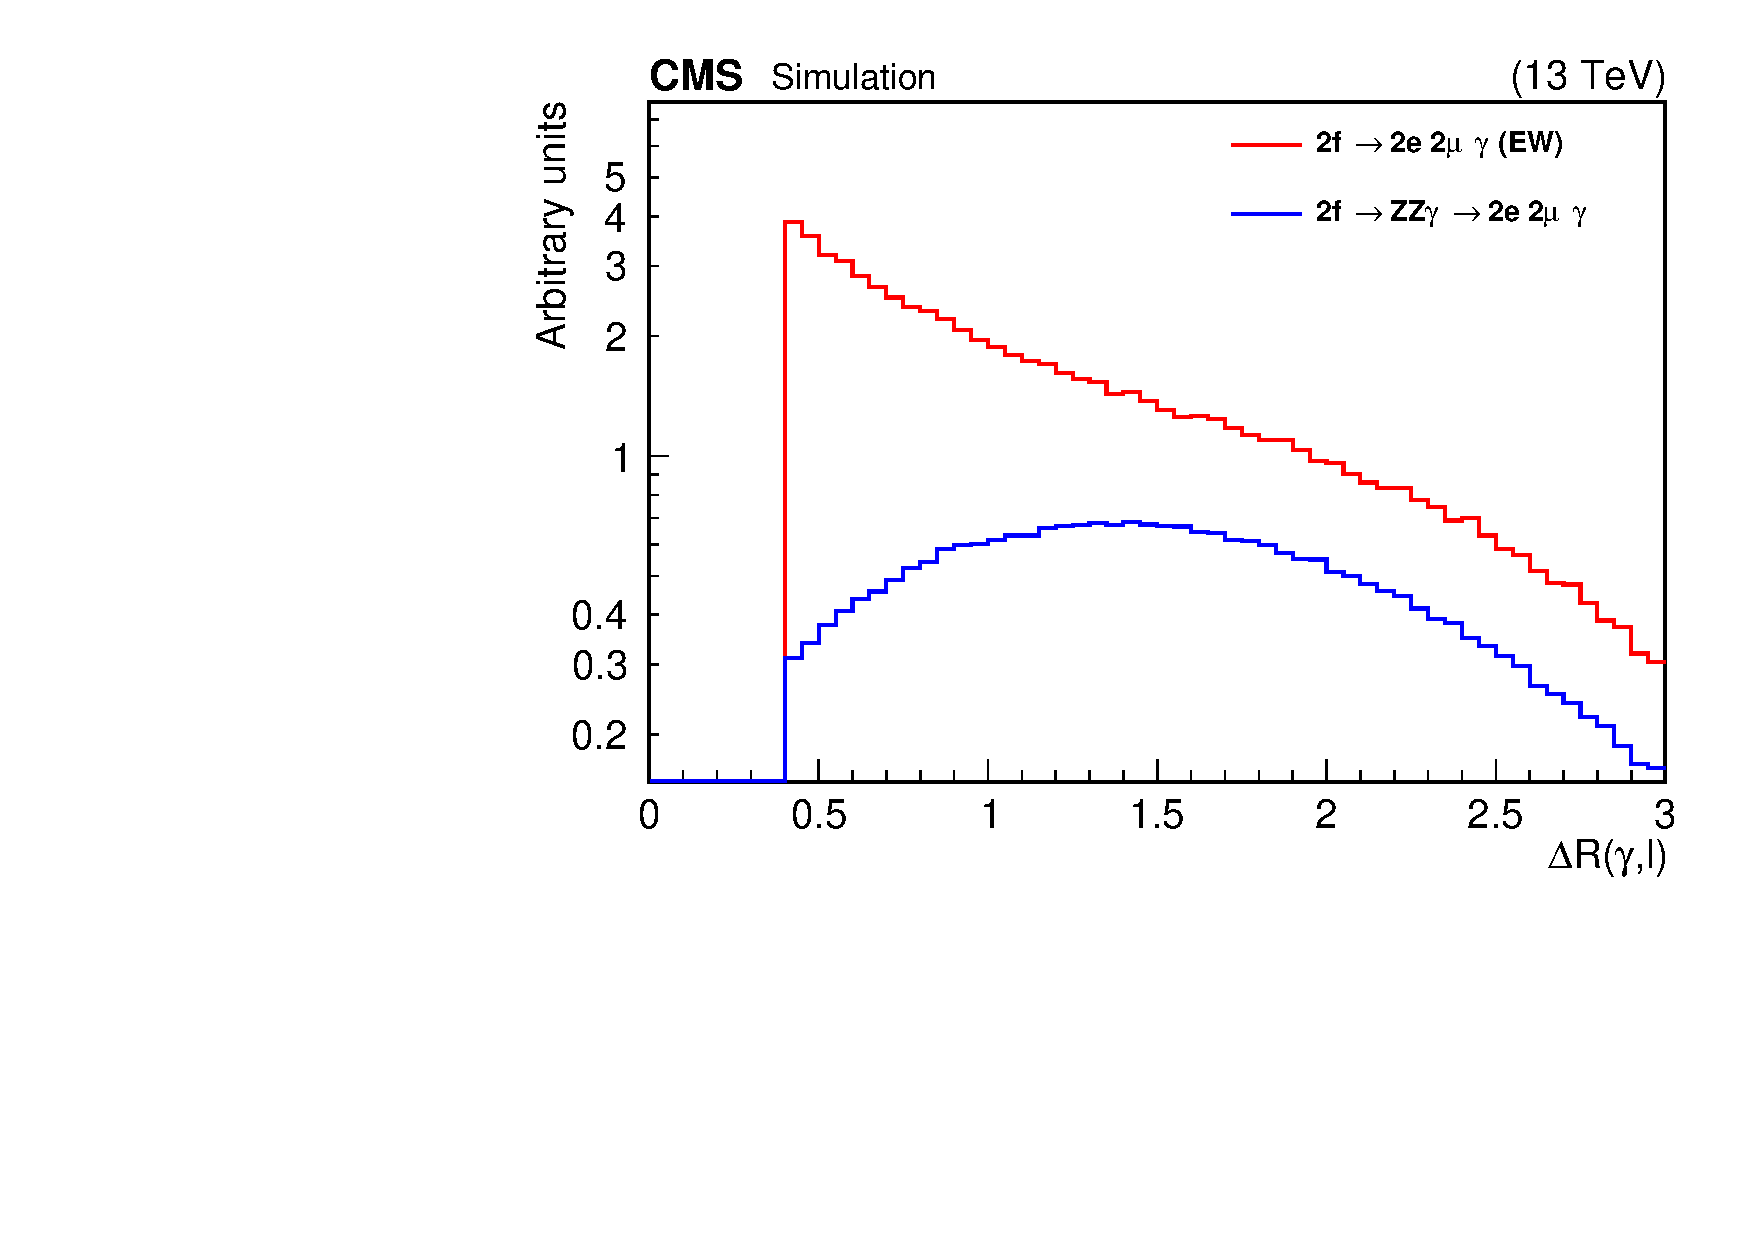
\includegraphics[width=.45\textwidth]{genstudy_dRlCloserG.pdf}}\hfill\mbox{}
  \caption{Invariant mass of the same-flavour opposite-sign lepton pairs
    and $\DR$ distance between the photon and the closest lepton
  in the two MC samples produced for the study of the fraction of FSR events in the $\Pp\Pp \to 4\Pl\PGg$ process.}
  \label{fig:genstudy}
\end{figure}

The distribution of the invariant mass of the dilepton pairs $m_{\Pl\Pl}$ after the application of the cut
$\DR(\Pl,\PGg) > 0.5$ is shown in Figure~\ref{fig:genstudy_mll_dRl0p5}.
Figure~\ref{fig:genstudy_ptGamma_cuts} displays the distribution of the  transverse momentum of the photon
after applying also the cut $m_{\Pl\Pl} > 81\GeVcc$.
The transverse momentum of FSR photons tends to be lower,
and it becomes almost zero above $\approx 70\GeVc$.
However only a fraction of the events in both samples are in the high momentum tail.

The yields before and after the application of the cuts are reported in Table~\ref{tab:genstudy_yields}.
The cuts result in a reduction
of 36\usep\% and 9\usep\% of the yield in the inclusive and constrained samples respectively.
The FSR component, which is the difference of the two, is reduced by 51\usep\%.

\begin{figure}
  \centering\hfill
  \subfigure [Dilepton invariant mass] {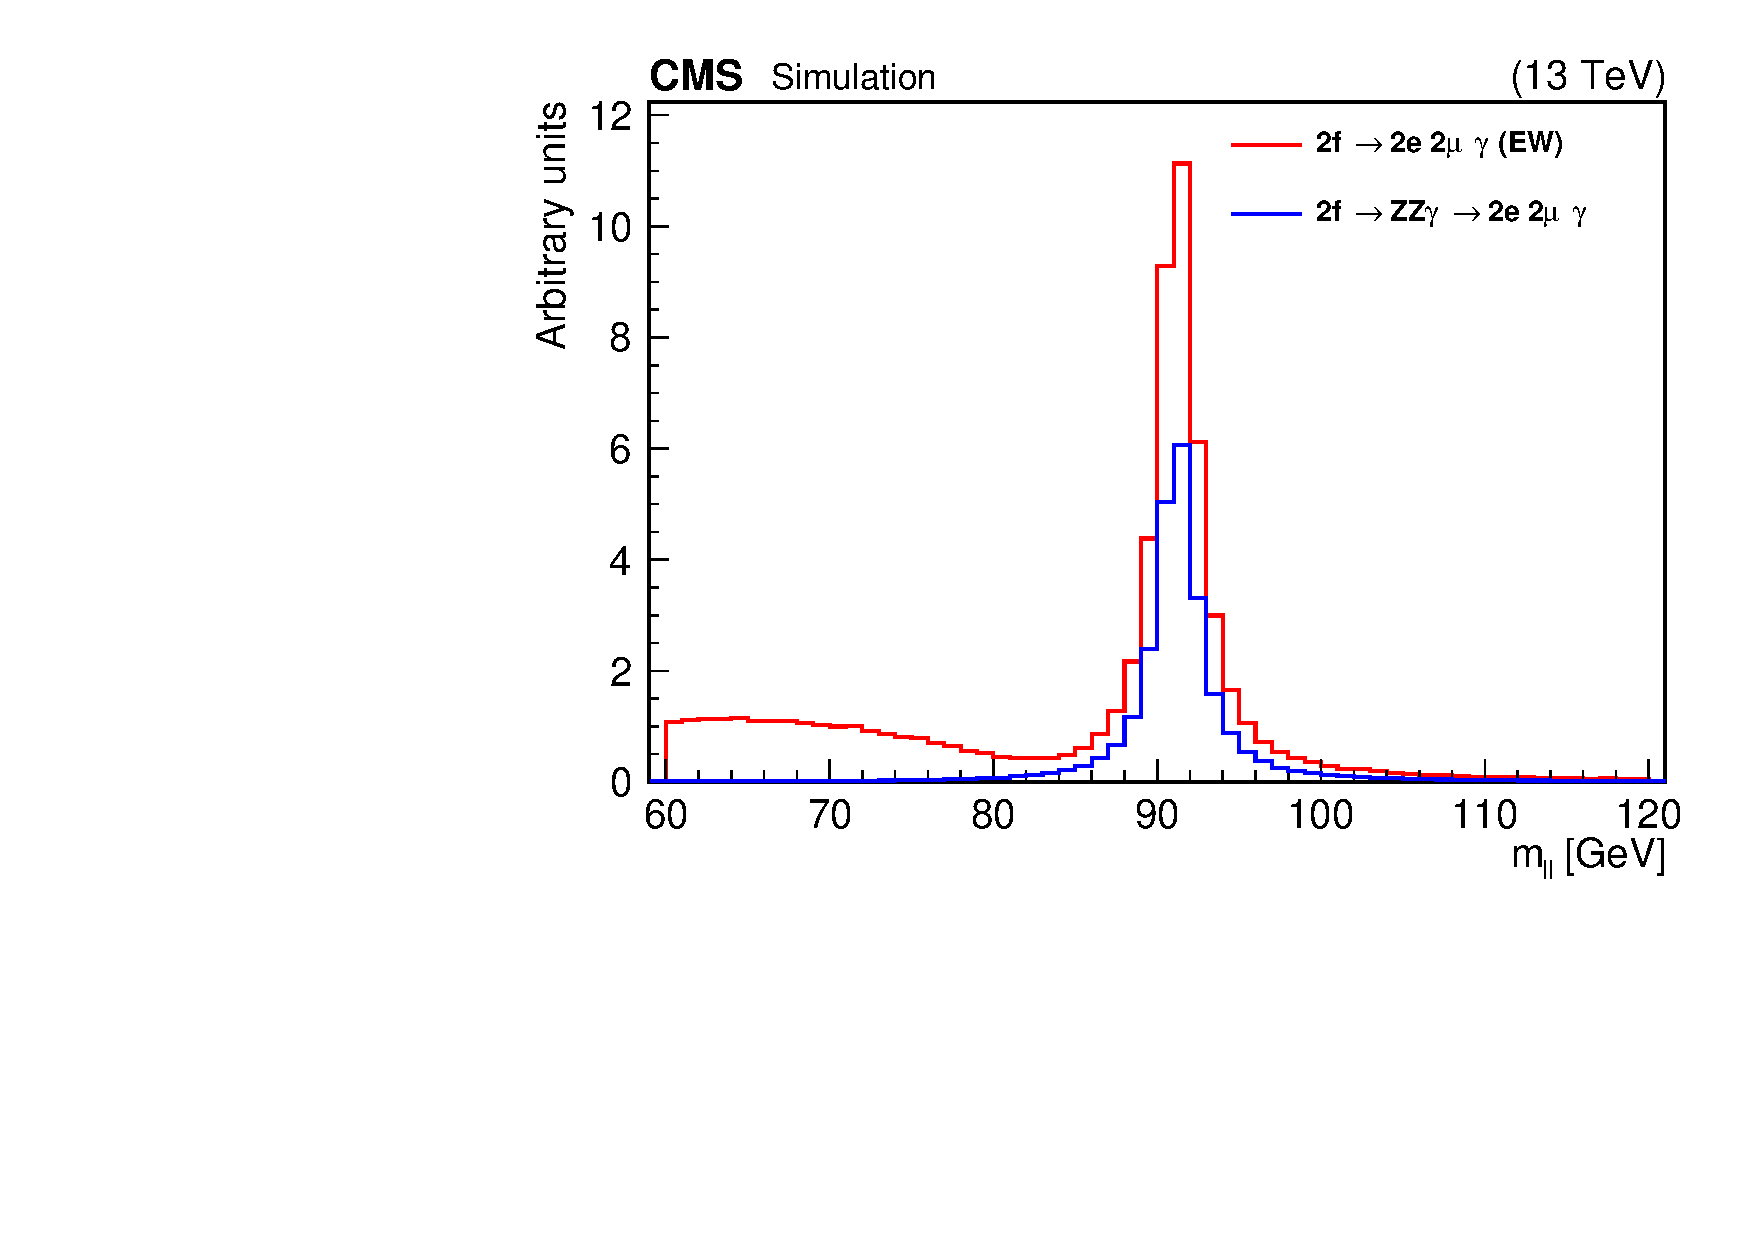
\includegraphics[width=.45\textwidth]{genstudy_mll_dRl0p5.pdf} \label{fig:genstudy_mll_dRl0p5}}\hfill
  \subfigure [Photon transverse momentum] {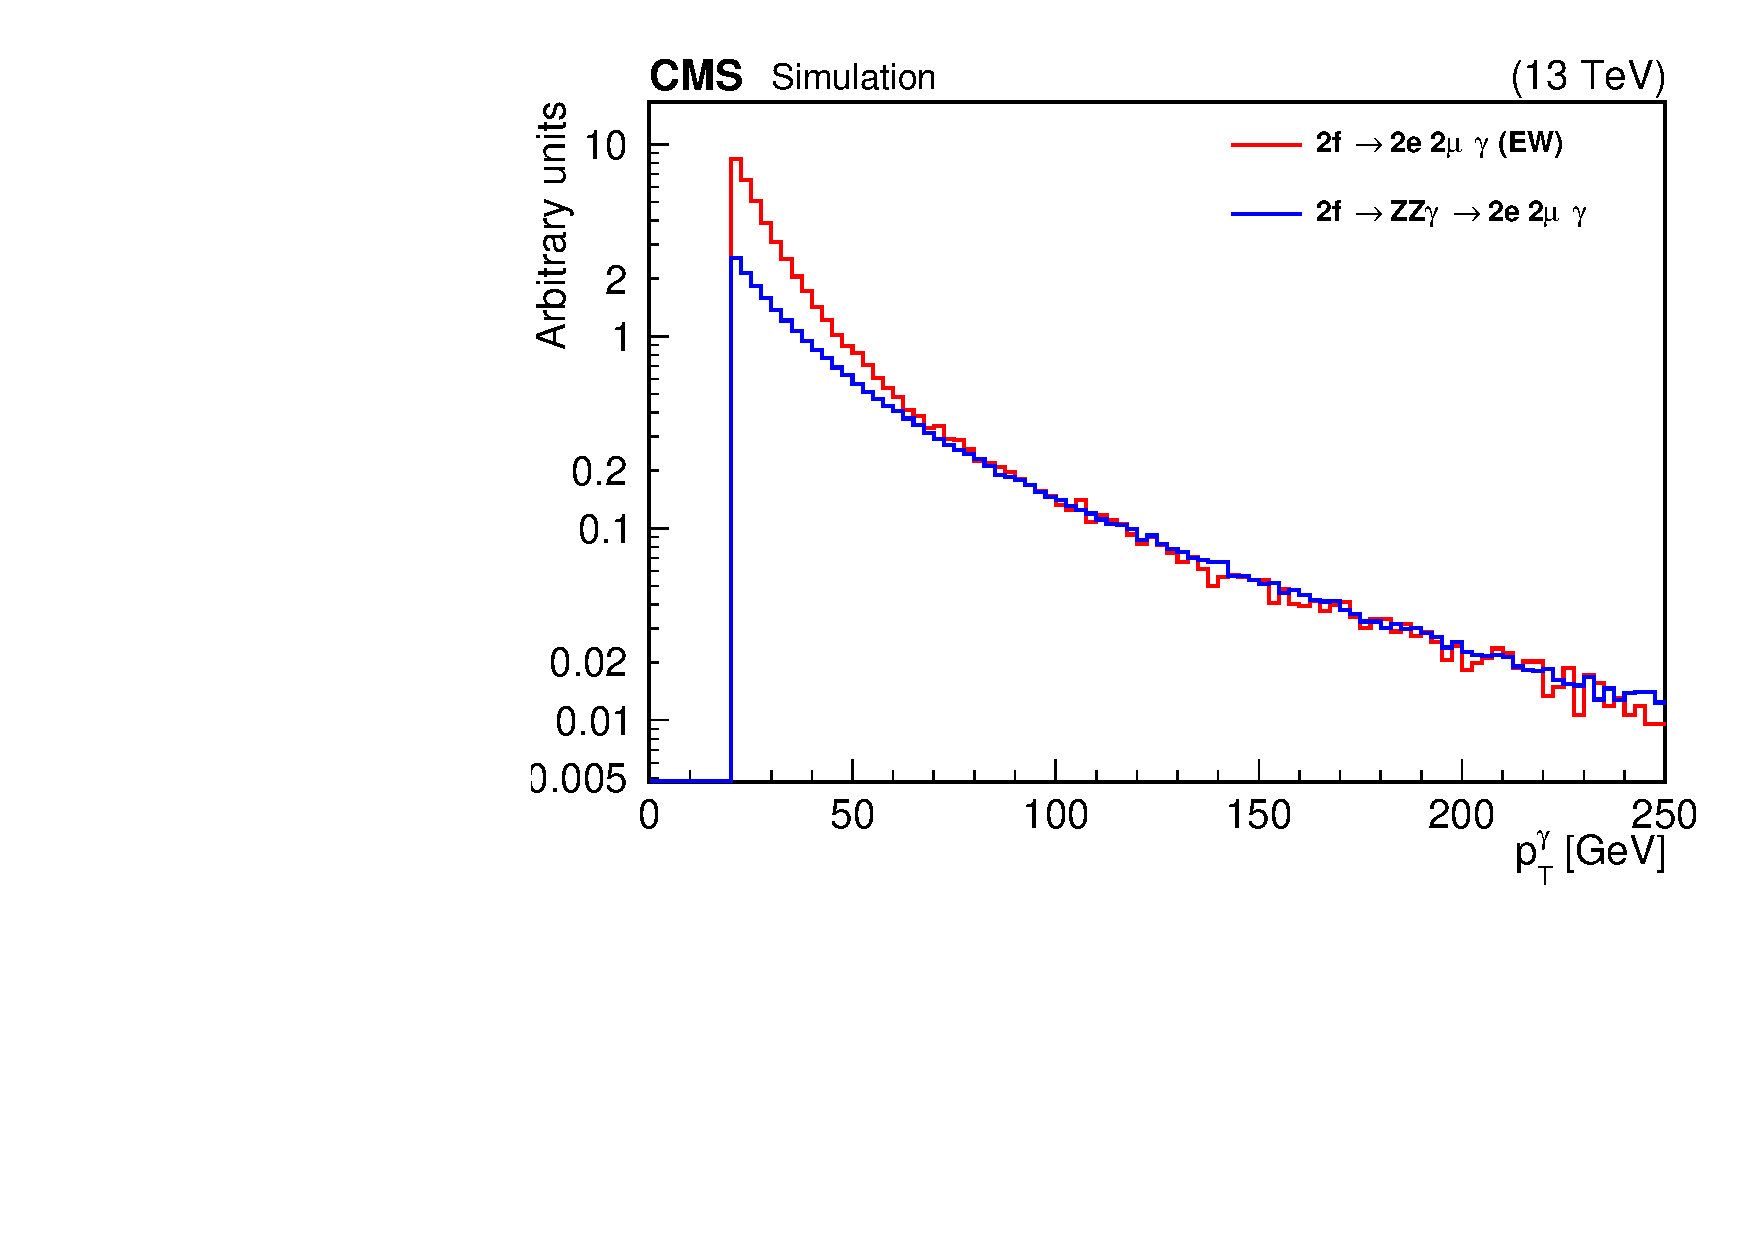
\includegraphics[width=.45\textwidth]{genstudy_ptGamma_cuts.pdf} \label{fig:genstudy_ptGamma_cuts}}\hfill\mbox{}
  \caption{
    Invariant mass of the same-flavour opposite-sign lepton pairs
    (left) after requiring $\DR(\Pl,\PGg) > 0.5$;
    $\DR$ distance between the photon and the closest lepton (right)
    after the additional application of the cut on the minimum dilepton invariant mass.
  }
  \label{fig:genstudy_cuts}
\end{figure}

\begin{table}
  \centering
  \caption{Number of events in the inclusive and constrained samples (and their difference) after applying the cuts to suppress the FSR component.}
  \label{tab:genstudy_yields}
  \begin{tabular}{l r@{}r r@{}r r@{}r}
    \toprule
    Cut                   & \multicolumn{2}{c}{inclusive} & \multicolumn{2}{c}{constrained} & \multicolumn{2}{c}{difference}\\
    \midrule
    %%None (not even dRl0p4)&         74.488& (100\usep\%)  &         27.279&   (100\usep\%)  &       47.202& (100\%) \\
    None                  &         74.5  & (100\usep\%)  &         26.1  &   (100\usep\%)  &       48.4  & (100\%) \\
    $\DR(\Pl,\PGg) > 0.5$ &         67.0  & ( 90\usep\%)  &         25.4  &    (93\usep\%)  &       41.6  & ( 86\%) \\
    $m_{ll} > 81\GeV$     &         51.0  & ( 68\usep\%)  &         25.5  &    (98\usep\%)  &       25.5  & ( 53\%) \\
    Both cuts             &         47.8  & ( 64\usep\%)  &         24.9  &    (91\usep\%)  &       22.9  & ( 47\%) \\
    \bottomrule
  \end{tabular}
\end{table}

After the application of the cuts, the fraction of events of the second sample,
where the photon is forced to be attached to an initial-state fermion line,
is 52\usep\% of the total of the first sample, compared to the initial 35\usep\%.
